\documentclass[]{article}
\usepackage[letterpaper,margin=0.0cm,left=7.25cm]{geometry}
\usepackage{tikz}
\usepackage{pgfplots}
\pgfplotsset{compat=1.10}
\usepgfplotslibrary{fillbetween}
\usetikzlibrary{calc}
\usepackage[absolute]{textpos}
%\usepackage[cm]{fullpage}
\usepackage{enumerate}
\usepackage{multicol}
\usepackage{amsmath}
\usepackage{amssymb}
\usepackage{graphicx}
\usepackage{xcolor}
\usepackage{xstring}
\usetikzlibrary{shapes.geometric,calc}
\fboxsep0pt %to avoid the extra padding around the minipage


\usepackage{fancyhdr}
\setcounter{secnumdepth}{-1} %removes section numbers 
\newcommand{\EndLine}{ \\[0em]}
\newcommand{\point}[1]{\\[-.5em] \textbf{\fontsize{11pt}{12pt}\selectfont #1} \\[0em]}
\newcommand{\subpoint}[1]{\-\hspace{.2cm}  $\bullet$ \-\hspace{.05cm} \StrLeft{#1}{100} \\[0em]}
\newcommand{\Date}[1]{ \text{\fontsize{9pt}{12pt}\selectfont #1}}
\newcommand{\RighSideHeading}[1]{\vspace{-2em}\begin{center}\textbf{#1}\end{center}\vspace{-.5em}}
\newcommand{\Heading}[1]{\\{\large \textbf{#1}\\[-.5em]  \rule{14cm}{.1cm} \- \vspace{-.25cm}}}
\newcommand\score[2]{
\hspace*{-.5cm}
\pgfmathsetmacro\pgfxa{#1+1}
\tikzstyle{scorestars}=[star, star points=5, star point ratio=2.25, draw,inner sep=1.3pt,anchor=outer point 3]
  \begin{tikzpicture}[baseline]
    \foreach \i in {1,...,#2} {
    \pgfmathparse{(\i<=#1?"yellow":"gray")}
    \edef\starcolor{\pgfmathresult}
    \draw (\i*1.75ex,0) node[name=star\i,scorestars,fill=\starcolor]  {};
   }
  \end{tikzpicture}
}
%%%%%%%%%%%%%%%%%%%%%%%%%%%%%%%%%%%%%%%%%%%%%%%%%%%%%%%%%%%%%%%%%%%%%%%%%%%%%%%%%%%%%%
%%%%%%%%%%%%%%%%%%%%%%%%%%% begin document %%%%%%%%%%%%%%%%%%%%%%%%%%%%%%%%%%%%%%%%%%%
%%%%%%%%%%%%%%%%%%%%%%%%%%%%%%%%%%%%%%%%%%%%%%%%%%%%%%%%%%%%%%%%%%%%%%%%%%%%%%%%%%%%%%

\begin{document}
\addtolength{\topmargin}{1in}
\pagestyle{empty} %removes page number

%Name
\begin{textblock}{6}(9,.25)
\begin{center}
\begin{Huge}
\bf
Trevor M. Decker\\
\end{Huge}
tdecker@andrew.cmu.edu \hspace{1cm} U.S. Citizen \\
1109 greenridge Lane Pittsburgh PA, 15220\\
\end{center}
\end{textblock}

% decided to not include an objective 
%&\text{Objective }&&\text{To obtain a fulltime position at a company that does cool important %things that matter where I can utilize my skills and passione in engineering and robotics to % work with a fun team to change the world.}\\[.5em]
%
%
%Work Eperience
\-\
\vspace*{-.7cm}
 \Heading{Employment History}\\
\point{Research Assistant, CMU Field Robotics Center (FRC) \Date{2011 - Current}}
\subpoint{Assisted with software and hardware maintenance/development of 10+ robots} 
\subpoint{Built multirobot localization algorithms in low infrastructure environments }
\subpoint{Robots collaboratively move parts in intracuite assembly}
\subpoint{Developed Kalman filter  and EKF for sensor fusion}
\subpoint{Added vision system to robot to allow for automated initialization }
%
%
%%%%%%%%%%%%%%%%%%%%%%%%%%%%%%%%%%%%%%%%%%%%%%%%%%%%%%%%%%%%%%%%%%%%%%%%%%%%%%%%%%%%%%%%%%%%%%
%
%
%Amazon Prime Air
\point{Intern, Amazon Prime Air \Date{Summer 2015}}  
\subpoint{developed algorithms and an embeded system controller }
\subpoint{Team is applying for multiple pattents based on my work}
\subpoint{Finish Internship project 1 month early delling with vision sensor placement}
\subpoint{Helped another intern finish a second project}
\subpoint{My development of less expensive sensor may save team  75,000+ per robot}
%
%
%%%%%%%%%%%%%%%%%%%%%%%%%%%%%%%%%%%%%%%%%%%%%%%%%%%%%%%%%%%%%%%%%%%%%%%%%%%%%%%%%%%%%%%%%%%%%%
%
%
%Volkswagen
\point{Intern, Volkswagen Electronics Research Laboratory \Date{Summer 2014}} 
\subpoint{Developed scalable architecture for sensor extrinsic calibration verification}
\subpoint{Upgraded legacy code to work with new system interface}
\subpoint{Participated in and helped organize Computer Vision reading group}
\subpoint{Won 3rd place at internal hackathon}
%
%
%
%
 \point{Introduction to robotics TA \Date{Spring 2014,2015}}
 \subpoint{Co-created final lab for class 2013}
 \subpoint{Designed bayes filter locilisation lab, robots solve the lost robot problem}
 \subpoint{Taught locilisation/state estimation lecture for proffsor}
 \subpoint{Helped write and grade midterm/final 2014,2015}
%
%
%
%
%
%
%Projects
%
%
%%GOS
 \Heading{Activities}\\
 \point{Mentor, Girls Of Steel FIRST Robotics Team 3504 \Date{2011 - 2013}}
%
 \subpoint{Mentored CMU sponsored robotics team of 40+ high school girls}
 \subpoint{Directly mentored programmers, who won regional innovation in control  award}
 \subpoint{Co-taught Java programming course for students}
%
%%%%%%%%%%%%%%%%%%%%%%%%%%%%%%%%%%%%%%%%%%%%%%%%%%%%%%%%%%%%%%%%%%%%%%%%%%%%%%%%%%%%%%%%%%
%
%Mecatronics 
 \point{Mecatronic Design, Spring 2015}
 \subpoint{recived "Coolest Coolness Factor" award, designed to move between windows}
 \subpoint{Designed/built 5 degree of freedom robot to clean arbatray skyscrapper windows}
 \subpoint{built passive complient gravity assited attachment to window}
 \subpoint{robot would stay on the window in the event of power loss, or slight missalignment}
 \subpoint{Implemented vision system which can locilise robot relative to the windows frame}

%
%%%%%%%%%%%%%%%%%%%%%%%%%%%%%%%%%%%%%%%%%%%%%%%%%%%%%%%%%%%%%%%%%%%%%%%%%%%%%%%%%%%%%%%%%%%
%
%RoboBuggy
\-\ 
\vspace*{-.5cm} 
\point{Robotic Buggy \Date{2013 - Current}} 
\subpoint{Creating a robot which can autonumusly compete in a gravity race at CMU}
\subpoint{Lead Software Team (manage 8+ people) Responsible for all software and firmware }
\subpoint{Developed a scalable real time aractecure for mapping,path planing, and loclisation}
\subpoint{Wrote motion model and observation model for GPS, IMU, encoders, cameras, ...}
\subpoint{Built road lane and building feature detectors to help extract robot’s state}
%
%Apex
%
\point{Apex Buggy Team \Date{2011 - Current}}  
\subpoint{Relay race at CMU with human driven carbon fiber carts built by students} 
\subpoint{Co-founded team as a freshman (now has 40+ members)}
\subpoint{Helped write constitution, and raised over 3,000 for team}
\subpoint{Lead mechanic during 2013 Races, no mechanical faults and won our heat}
%
%
%
%
%
  \Heading{Distinctions}  \\[.6em]
\subpoint{Resident Assistant for 30+ visiting Chinese students for a 2 week robotics camp 2013}
\subpoint{Computer Technician, Diagnosed and repaired computers for 650+ students 2009 - 2011}
\subpoint{Black Belt,Tang Soo Do Karate}
\subpoint{Volunteer of the Year, 2007,Carnegie Science Center 200+ hours} 
\subpoint{National Honors Society, President,City Charter High School} 





\begin{textblock}{3}(-.5,0)
\colorbox{lightgray}
{
\begin{minipage}{7cm}
\hspace{.25cm}
\begin{minipage}{6.5cm}
\-\
\\[8em]
\RighSideHeading{Education}
\vspace{-.5cm}
%
%
\-\ \\
Carnagie Mellon University (2011-2016)\\
Integrated Masters/Bacholers\\
In Electrical Computer Engineering\\
Minors in Computer Science, Robotics and Buissnes Administration\\
\vspace{-.5cm}
%
%
\rule{6cm}{.05cm}
\-\ \\[.5cm]
\RighSideHeading{Relevant classes}
$\bullet$ Real Time Embeded Systems: \\
designed working RTOS\\	
%
$\bullet$ Embeded Controls: \\
programmed stable inverted pendulum\\
%
$\bullet$ Robot Kinematics And Dynamics: 
developed kalman filter for paramater estimation\\
%
$\bullet$ Computer Vision:\\
designed optical text recontion system\\
Distributed Embeded Systems:\\
 Currently enrolled\\
 %
$\bullet$ Statistical Techniques in Robotics: \\
Currently enrolled\\
%
$\bullet$ Machine Learning: Currently enrolled\\
%
%
%
%
%
%
\rule{6cm}{.05cm}
\-\ \\
\vspace{-1em}
\begin{flushright}
\vspace*{.3cm}
\RighSideHeading{Programming}
\vspace*{-.2cm}
\begin{multicols}{2}
\vspace{.5em}
Matlab \score{5}{5}\\
C   \score{4}{5}\\
C++ \score{3.5}{5}\\
Java \score{4}{5}\\
Python \score{3}{5}\\
Verilog \score{1}{5}\\
HTML \score{3}{5} \\
PHP \score{2}{5} \\
JavaScript \score{2}{5}\\
SML \score{2}{5} \\
Labview \score{1}{5}\\
LaTex \score{3}{5}\\
\end{multicols}
%
%
%
\vspace{0cm}
\RighSideHeading{Libraries}
\begin{multicols}{2}
\vspace*{-1cm}
ROS \score{3}{5} \\
Free RTOS \score{2}{5} \\
OpenCV \score{2}{5}\\
PCL \score{1}{5} \\
\end{multicols}
%
%
\vspace{0cm}
\RighSideHeading{Software}
%\begin{multicols}{2}
\vspace{-.3cm}
Adobe Premiere \score{2}{5}\\
SolidWorks \score{3}{5}\\
linux \score{3}{5}\\
%\end{multicols}
%
%
\vspace{1em}
\RighSideHeading{Mechanical}
%\begin{multicols}{2}
\vspace{-.5em}
Mill \score{3}{5}\\
Lathe \score{2}{5}\\
3d printer \score{4}{5}\\
laser cutter \score{3}{5}\\
Carbon Fiber \score{1}{5}\\
\rule{6cm}{.05cm}\\
\end{flushright}
\begin{figure}
    \centering
\includegraphics[scale=.002]{qr}\\
Scan to see some of my work\\
\end{figure}
\end{minipage}
\\[4em]
\end{minipage}}
\end{textblock}
%
%
%
%
% top triangle
%
%
\begin{textblock}{3}(-.5,0)
\-\
\\[-1em]
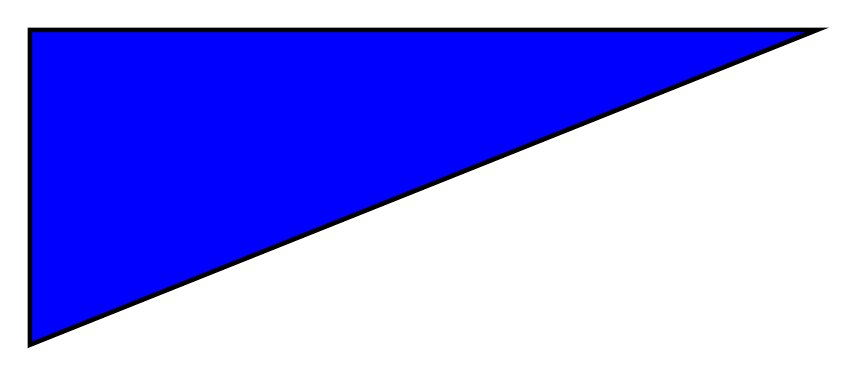
\begin{tikzpicture}
      \draw [ultra thick, draw=black, fill=blue, opacity=1.0]
	  (0,0) --     
      (0,4) --
      (10,4)--
       cycle;
\end{tikzpicture}
\end{textblock}
%
%
%
% bottom right triangle
%
%
\begin{textblock}{3}(11.5,15)
\-\
\\[-1em]
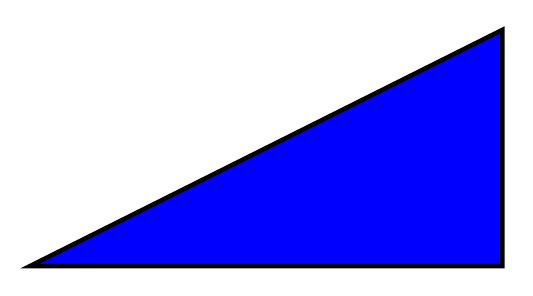
\begin{tikzpicture}
% Create random(ish) points

%\foreach \i in {1,...,26}
%  \fill [opacity=0.5] (360/26*\i:1+i*1) circle [radius=.1] coordinate (mark-\i);
% Join them up
%\fill [opacity=0.5,blue]
 % (mark-1) \foreach \i in {2,...,26}{ -- (mark-\i) } -- cycle;
      \draw [ultra thick, draw=black, fill=blue, opacity=1.0]
	  (0,0) --     
      (6,0) --
      (6,3)--
       cycle;
\end{tikzpicture}
\end{textblock}
%
%
% total page overlay
%
%
\begin{textblock}{3}(-.4,0)
\begin{tikzpicture}
      \draw [ultra thick, draw=black, fill=red, opacity=0.0]
	  (0in,0in) --     
      (0in,-11.5in) --
      (8.5in,-11.5in) --     
      (8.5in,0in) --
      cycle;
\end{tikzpicture}
\end{textblock}
%
%
% Printable area overlay
%
%  THis section is for making sure that the entrie document is in the printable region
%
\begin{textblock}{3}(-.4,0)
\begin{tikzpicture}
      \draw [ultra thick, draw=black, fill=blue, opacity=0.0]
	  (0in,0in) 
	  (.15in,-.22in)-- 
      (.15in,-10.82in) --
      (8.35in,-10.82in) --
      (8.35in,-.22in) --
      cycle;
\end{tikzpicture}
\end{textblock}
\end{document}
